% Created by tikzDevice version 0.10.1.2 on 2018-04-18 11:15:26
% !TEX encoding = UTF-8 Unicode
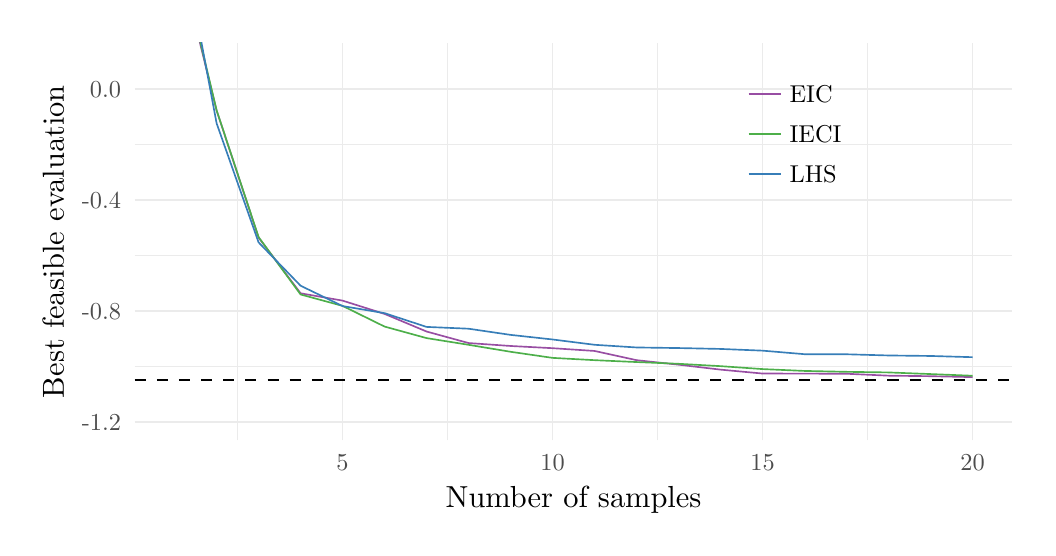
\begin{tikzpicture}[x=1pt,y=1pt]
\definecolor{fillColor}{RGB}{255,255,255}
\path[use as bounding box,fill=fillColor,fill opacity=0.00] (0,0) rectangle (361.35,180.67);
\begin{scope}
\path[clip] ( 38.67, 31.53) rectangle (355.85,175.17);
\definecolor{drawColor}{gray}{0.92}

\path[draw=drawColor,line width= 0.3pt,line join=round] ( 38.67, 58.15) --
	(355.85, 58.15);

\path[draw=drawColor,line width= 0.3pt,line join=round] ( 38.67, 98.33) --
	(355.85, 98.33);

\path[draw=drawColor,line width= 0.3pt,line join=round] ( 38.67,138.51) --
	(355.85,138.51);

\path[draw=drawColor,line width= 0.3pt,line join=round] ( 75.85, 31.53) --
	( 75.85,175.17);

\path[draw=drawColor,line width= 0.3pt,line join=round] (151.73, 31.53) --
	(151.73,175.17);

\path[draw=drawColor,line width= 0.3pt,line join=round] (227.61, 31.53) --
	(227.61,175.17);

\path[draw=drawColor,line width= 0.3pt,line join=round] (303.49, 31.53) --
	(303.49,175.17);

\path[draw=drawColor,line width= 0.6pt,line join=round] ( 38.67, 38.06) --
	(355.85, 38.06);

\path[draw=drawColor,line width= 0.6pt,line join=round] ( 38.67, 78.24) --
	(355.85, 78.24);

\path[draw=drawColor,line width= 0.6pt,line join=round] ( 38.67,118.42) --
	(355.85,118.42);

\path[draw=drawColor,line width= 0.6pt,line join=round] ( 38.67,158.60) --
	(355.85,158.60);

\path[draw=drawColor,line width= 0.6pt,line join=round] (113.79, 31.53) --
	(113.79,175.17);

\path[draw=drawColor,line width= 0.6pt,line join=round] (189.67, 31.53) --
	(189.67,175.17);

\path[draw=drawColor,line width= 0.6pt,line join=round] (265.55, 31.53) --
	(265.55,175.17);

\path[draw=drawColor,line width= 0.6pt,line join=round] (341.43, 31.53) --
	(341.43,175.17);
\definecolor{drawColor}{RGB}{152,78,163}

\path[draw=drawColor,line width= 0.6pt,line join=round] ( 60.90,180.67) --
	( 68.27,150.75) --
	( 83.44,104.81) --
	( 98.62, 84.69) --
	(113.79, 82.04) --
	(128.97, 77.23) --
	(144.15, 70.87) --
	(159.32, 66.71) --
	(174.50, 65.65) --
	(189.67, 64.85) --
	(204.85, 63.85) --
	(220.03, 60.52) --
	(235.20, 58.89) --
	(250.38, 57.10) --
	(265.55, 55.69) --
	(280.73, 55.66) --
	(295.90, 55.61) --
	(311.08, 54.92) --
	(326.26, 54.73) --
	(341.43, 54.40);
\definecolor{drawColor}{RGB}{77,175,74}

\path[draw=drawColor,line width= 0.6pt,line join=round] ( 61.14,180.67) --
	( 68.27,150.82) --
	( 83.44,105.01) --
	( 98.62, 84.26) --
	(113.79, 80.13) --
	(128.97, 72.66) --
	(144.15, 68.49) --
	(159.32, 66.07) --
	(174.50, 63.55) --
	(189.67, 61.35) --
	(204.85, 60.52) --
	(220.03, 59.84) --
	(235.20, 59.21) --
	(250.38, 58.36) --
	(265.55, 57.30) --
	(280.73, 56.63) --
	(295.90, 56.31) --
	(311.08, 56.09) --
	(326.26, 55.50) --
	(341.43, 54.89);
\definecolor{drawColor}{RGB}{55,126,184}

\path[draw=drawColor,line width= 0.6pt,line join=round] ( 61.79,180.67) --
	( 68.27,146.12) --
	( 83.44,103.08) --
	( 98.62, 87.42) --
	(113.79, 80.07) --
	(128.97, 77.51) --
	(144.15, 72.54) --
	(159.32, 71.89) --
	(174.50, 69.66) --
	(189.67, 68.00) --
	(204.85, 66.08) --
	(220.03, 65.11) --
	(235.20, 64.90) --
	(250.38, 64.58) --
	(265.55, 63.96) --
	(280.73, 62.68) --
	(295.90, 62.65) --
	(311.08, 62.22) --
	(326.26, 62.04) --
	(341.43, 61.60);
\definecolor{drawColor}{RGB}{0,0,0}

\path[draw=drawColor,line width= 0.6pt,dash pattern=on 4pt off 4pt ,line join=round] ( 38.67, 53.43) -- (355.85, 53.43);
\end{scope}
\begin{scope}
\path[clip] (  0.00,  0.00) rectangle (361.35,180.67);
\definecolor{drawColor}{gray}{0.30}

\node[text=drawColor,anchor=base east,inner sep=0pt, outer sep=0pt, scale=  0.88] at ( 33.72, 35.03) {-1.2};

\node[text=drawColor,anchor=base east,inner sep=0pt, outer sep=0pt, scale=  0.88] at ( 33.72, 75.21) {-0.8};

\node[text=drawColor,anchor=base east,inner sep=0pt, outer sep=0pt, scale=  0.88] at ( 33.72,115.39) {-0.4};

\node[text=drawColor,anchor=base east,inner sep=0pt, outer sep=0pt, scale=  0.88] at ( 33.72,155.57) {0.0};
\end{scope}
\begin{scope}
\path[clip] (  0.00,  0.00) rectangle (361.35,180.67);
\definecolor{drawColor}{gray}{0.30}

\node[text=drawColor,anchor=base,inner sep=0pt, outer sep=0pt, scale=  0.88] at (113.79, 20.52) {5};

\node[text=drawColor,anchor=base,inner sep=0pt, outer sep=0pt, scale=  0.88] at (189.67, 20.52) {10};

\node[text=drawColor,anchor=base,inner sep=0pt, outer sep=0pt, scale=  0.88] at (265.55, 20.52) {15};

\node[text=drawColor,anchor=base,inner sep=0pt, outer sep=0pt, scale=  0.88] at (341.43, 20.52) {20};
\end{scope}
\begin{scope}
\path[clip] (  0.00,  0.00) rectangle (361.35,180.67);
\definecolor{drawColor}{RGB}{0,0,0}

\node[text=drawColor,anchor=base,inner sep=0pt, outer sep=0pt, scale=  1.10] at (197.26,  7.44) {Number of samples};
\end{scope}
\begin{scope}
\path[clip] (  0.00,  0.00) rectangle (361.35,180.67);
\definecolor{drawColor}{RGB}{0,0,0}

\node[text=drawColor,rotate= 90.00,anchor=base,inner sep=0pt, outer sep=0pt, scale=  1.10] at ( 13.08,103.35) {Best feasible evaluation};
\end{scope}
\begin{scope}
\path[clip] (  0.00,  0.00) rectangle (361.35,180.67);
\definecolor{drawColor}{RGB}{152,78,163}

\path[draw=drawColor,line width= 0.6pt,line join=round] (260.52,156.74) -- (272.09,156.74);
\end{scope}
\begin{scope}
\path[clip] (  0.00,  0.00) rectangle (361.35,180.67);
\definecolor{drawColor}{RGB}{77,175,74}

\path[draw=drawColor,line width= 0.6pt,line join=round] (260.52,142.29) -- (272.09,142.29);
\end{scope}
\begin{scope}
\path[clip] (  0.00,  0.00) rectangle (361.35,180.67);
\definecolor{drawColor}{RGB}{55,126,184}

\path[draw=drawColor,line width= 0.6pt,line join=round] (260.52,127.83) -- (272.09,127.83);
\end{scope}
\begin{scope}
\path[clip] (  0.00,  0.00) rectangle (361.35,180.67);
\definecolor{drawColor}{RGB}{0,0,0}

\node[text=drawColor,anchor=base west,inner sep=0pt, outer sep=0pt, scale=  0.88] at (275.34,153.71) {EIC};
\end{scope}
\begin{scope}
\path[clip] (  0.00,  0.00) rectangle (361.35,180.67);
\definecolor{drawColor}{RGB}{0,0,0}

\node[text=drawColor,anchor=base west,inner sep=0pt, outer sep=0pt, scale=  0.88] at (275.34,139.26) {IECI};
\end{scope}
\begin{scope}
\path[clip] (  0.00,  0.00) rectangle (361.35,180.67);
\definecolor{drawColor}{RGB}{0,0,0}

\node[text=drawColor,anchor=base west,inner sep=0pt, outer sep=0pt, scale=  0.88] at (275.34,124.80) {LHS};
\end{scope}
\end{tikzpicture}
